\chapter{Input/Output scheduling}
\section{Introduction, hard drives technology}

Algorithms for I/Os scheduling in use today are motivated by mechanical hard drives technology.
A mechanical hard drive is made :
\begin{itemize}
  \item platters (rotating) on which data is stored.
  \item arm to move r/w heads.
  \item r/w head at the end of the arm.
\end{itemize}

\begin{figure}[h!]
  \begin{center}
    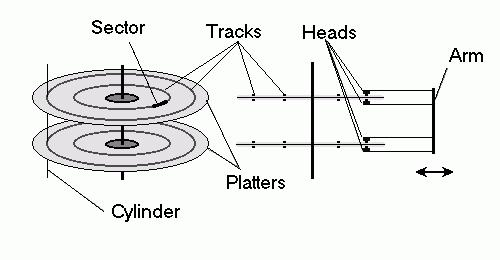
\includegraphics{hard_drive_picture.jpg}
  \end{center}
\end{figure}

%place hard drive picture here
To perform an access to a specific sector :
\begin{itemize}
  \item move the arm to the proper track
  $=>$ takes time: depends on the engine moving the arm.
  \item wait for the desired sector
   $=>$ takes time: depends on the rotating speed of the platters.
  \item select the head and read or write
  $=>$ fast.
\end{itemize}

As a result, the access time to some sector will be :
\begin{itemize}
  \item fast: if the arm is already on the right track and the sector already under the r/w head. (about 125 MB/s $=>$ 500 nanoseconds to get 4 bytes).
  It is the bandwidth of sequential accesses.
  \item slow: otherwise (about 10 ms to get 4 bytes : there is a 20 000 factor).
  It is the latency of a random access.
  
\end{itemize}

Usually, sequential accesses can reach full bandwidth with a small degradation on track change.
Latency is given on average, the exact latency depends on the istance of the arm from the track and on the sector position.

\section{I/Os scheduling}

The CPU is much faster than a hard disk, even at full bandwidth, there is a possibility to produce more I/O requests than the drive can handle

$=>$ queue of pending requests in the kernel

$=>$ optimizations: reordering, aggregation.

\subsection{FcFs (First come First served)}

\begin{figure}[h!]
  \begin{center}
    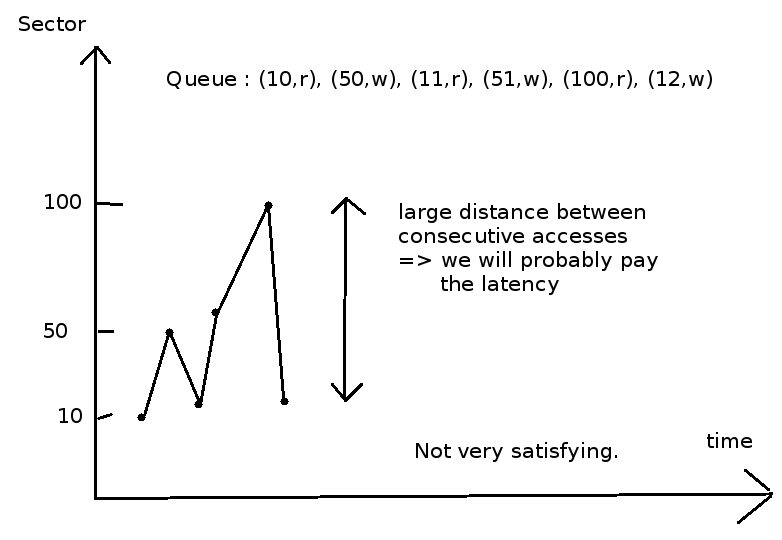
\includegraphics[width=0.6\textwidth]{fcfs.png}
  \end{center}
\end{figure}

\subsection{SSTF ( SSF, NBF)}

Shortest seek-time first of shorter seek first or nearest block first.

\begin{figure}[th!]
  \begin{center}
    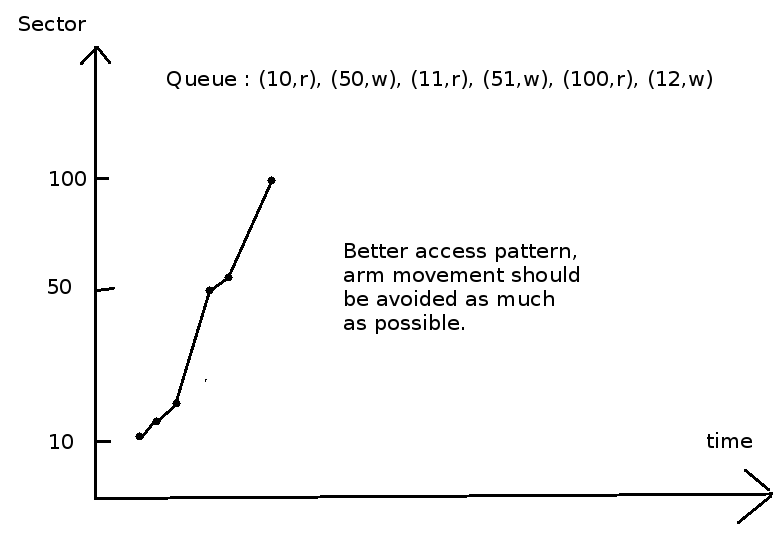
\includegraphics[width=0.6\textwidth]{sstf.png}
  \end{center}
\end{figure}

But :

\begin{itemize}
  \item adjacent accesses are the best if they are on the same track
  
  $=>$ should be improved by taking into account :
  
  
  (The geometry of the drive is not given to the OS). 
  \begin{itemize}
    \item number of tracks to cross
    \item time to wait for the sector once on the right track
  \end{itemize}
 
  
  $=>$ might be implemented in the disk itself (SCSI and SATA)
  
  \item starvation: if requests close the current head position arrive constantly.
  This is especially true for requests close to the ends of the disk.
\end{itemize}

\subsection{SCAN/LOOK/the elevator}

This algorithm serve requests in two phases :

\begin{itemize}
  \item first by increasing order of sector number
  \item secondly by decreasing order of sector number
\end{itemize}
Then it loops over these two phases.

\begin{figure}[h!]
  \begin{center}
    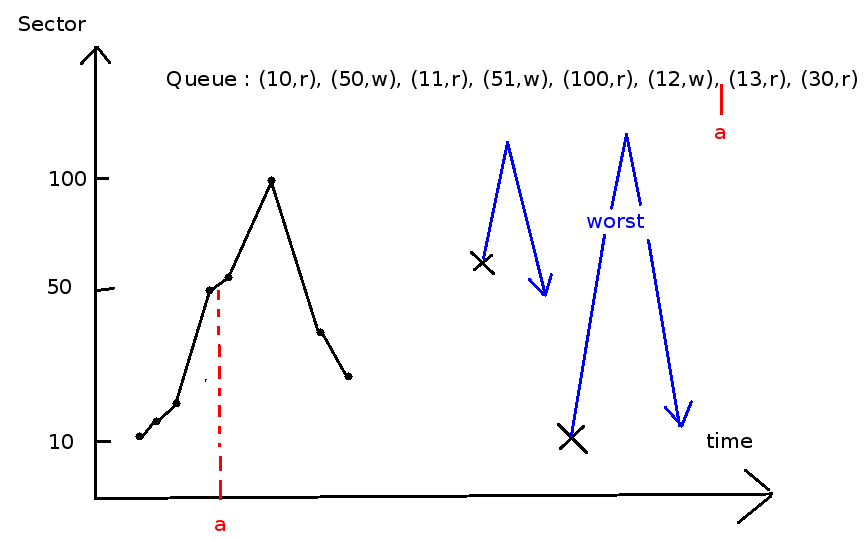
\includegraphics[width=0.8\textwidth]{elevator.png}
    \label{fig:1}
  \end{center}
\end{figure}

Advantages :

\begin{itemize}
  \item Some locality, close requests already in the queue will be grouped
  \item no starvation, the head moves strictly toward the last request in one direction.
\end{itemize}

Drawbacks :

\begin{itemize}
  \item accesses in the wrong direction are not necessarily efficient in the disk.
  \item requests on the middle of the disk have a better serving time $=>$ fairness issue
\end{itemize}

\subsection{Circular SCAN}

Serve request only by increasing sector number. Rewind to the request nearest to the beginning of the disk when the request with the largest sector number is served.
\begin{figure}[h!]
  \begin{center}
    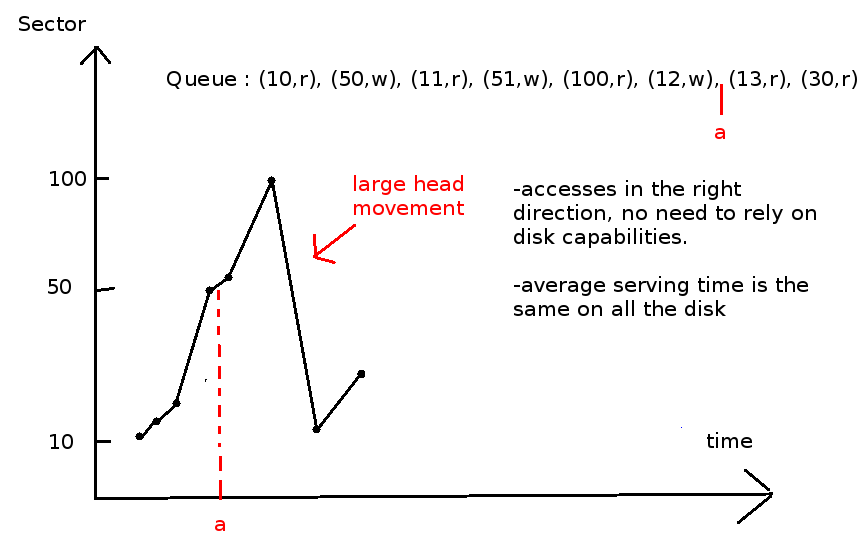
\includegraphics[width=0.8\textwidth]{circular.png}
    \caption{Circular Scan}
    \label{fig:2}
  \end{center}
\end{figure}
\subsection{Anticipatory scheduling}

Do not apply the work-first principle; when a process is performing a sequential access, all the requests are not necessarily in the queue.

The idea is to wait a little time after a request to let the opportunity to the served process to issue the next request

\subsection{Other strategies}
\begin{itemize}
  \item Deadline scheduling :
  requests are served by optimizing locality (SSTF with anticipatory waits) but are also associated with a deadline after which they will be served in priority.
  
  $=>$ no starvation
  
  \item fair queuing :
  each process has its own queue, the scheduler divied "fairly" the time during which a process can have its requests served.
\end{itemize}

\section{Conclusion}

These algorithms assume that :
\begin{itemize}
  \item sequential accesses are much faster than random ones (because of the 20 000 factor)
  \item it is worth spending time reordering requests ( very large gain).
  \item seek time depends on the distance between sectors.
\end{itemize}

But it is not completely true with newer technologies (SSD).

